\chapter{Implementação do Modelo}
\label{chapter:projeto}
    Este capítulo apresenta e detalha as implementações dos fluxos de execução hospedados no GitHub Actions e alguns dos testes unitários desenvolvidos, conforme mencionados no \autoref{chapter:proposta}.
    
    Para contextualização do modelo, bem como compreensão do ambiente de desenvolvimento, a \autoref{projeto:floripasat2} apresenta um detalhamento sobre a missão e como ela é dividia, em termos de desenvolvimento. Como discutido anteriormente, o FloripaSat-2 utiliza a filosofia Free Open Source Software, e portanto todos os módulos e subsistemas desenvolvidos estão publicados em repositórios abertos, no GitHub da missão. As seções \ref{projeto:eps}, \ref{projeto:ttc} e \ref{projeto:obdh} referenciam em seu texto os repositórios oficiais de cada um dos subsistemas desenvolvidos no SpaceLab.
     
    
    \section{FloripaSat-2}
    \label{projeto:floripasat2}
    
        Segundo Gonzales \textit{et. al.} (2019), "o \textit{software} de vôo de uma missão CubeSat constitui um dos elementos essenciais para garantia do sucesso da missão, já que é onde são implementados grande parte dos requisitos funcionais da missão". \cite{gonzales-2019}. Segundos os autores, é o que também permite que missões CubeSat sejam escaláveis e reutilizáveis.
        
        De fato, o FloripaSat-2 se beneficia destas propriedades. A missão é precedida pelo FloripaSat-1, lançado em dezembro de 2019, e como apresentado na \autoref{relacionados:marcelino2020-1}, segue a mesma metodologia e prática de desenvolvimento. Por consequencia, os módulos e substistemas, tanto \textit{hardware} como \textit{firmware} foram planejados para serem diretamente herdados do FloripaSat-1 ou atualizações de suas versões.
        
        Este trabalho foi em sua maioria focado nos subsistemas EPS 2.0 e OBDH 2.0 por estarem em estágios mais avançados de desenvolvimento, e os códigos-fonte discutidos e apresentados se encontram nos repositórios oficiais e públicos da missão, em \cite{eps2-github} e \cite{obdh2-github} respectivamente. Trechos relevantes do \textit{firmware} são apresentados e explicados neste capítulo, e apresentados em um contexto mais amplo nos anexos e apêndices ao final do documento. Por se tratarem de projetos relativamente grandes em questão de extensão de código, eles não foram anexados integralmente nesta monografia, que se beneficia do caráter público dos projetos do SpaceLab. Toda a implementação mencionada pode ser encontrada nos repositórios do FloripaSat-2 no GitHub\cite{floripasat2}.
        
        \subsection{EPS 2.0}
        \label{projeto:eps}
            O EPS 2 (\textit{electrical power system}) é responsável por coletar, armazenar e distribuir energia para o FloripaSat-2. A coleta de energia é feita através de 10 painéis solares posicionados ao longo da estrutura do satélite, e é armazenada em 4 baterias de íon de lítio. A distribuição de energia é feita através de conversores DC-AC. Tal qual o módulo desenvolvido para o FloripaSat-1\cite{marcelino2020-1} o EPS 2.0 possui um chip DS2775G+ utilizado para controlar carga e descarga da bateria, além de monitorar alguns parâmetros como corrente e tensão. O EPS, com base nessas informações, executa suas rotinas de distribuição de energia, decidindo quais módulos e quais funcionalidades devem permanecer em operação. O EPS 2 também é capaz de controlar a temperatura das baterias, e conta com sensores de temperatura e aquecedores.
            
            O projeto e implementação do EPS está disponível em seu repositório\cite{eps2-github}
            
        \subsection{TTC 2.0}
        \label{projeto:ttc}
            O módulo TTC 2 (Ou TT\&C, \textit{Telemetry, tracking \& Telecommand}) é o módulo de comunicação do FloripaSat-2. É função dele realizar a comunicação entre o satélite e a \textit{groundstation}. A comunicação com a estação terrestre será feita de duas maneiras, um sinal de \textit{beacon} e um de telemetria. 
            
            O \textit{beacon} transmite um sinal periódico contendo alguns dados básicos de identificação do satélite em conjunto com informações básicas de telemetria. O módulo de telemetria é o responsável pela comunicação de fato. Tém um módulo de comunicação bidimensional para receber telecomandos da Terra e transmitir os dados requisitados. O submódulo de telemetria é controlado por devices externos (como por exemplo o OBDH). 
            
            O projeto e a implementação do TTC 2 está disponível em seu repositório \cite{ttc2-github}.
        
        \subsection{OBDH 2.0}
        \label{projeto:obdh}
            O OBDH 2 (\textit{On-Board Data Handling}) é responsável pela sincronização as ações e o fluxo de dados entre os outros módulos do FloripaSat-2 e a groundstation. O OBDH organiza os dados em \textit{data frames} e transimte através do TTC, ou armazena em memória não-volátil para transimssão em outro momento. Dados recebidos da groundstation são captados pelo TTC e direcionados para o OBDH, que realiza a ação apropriada ou transmite para o módulo apropriado. 
            
            O OBDD também é responsável por sincronizar e fazer a interface entre os demais subsistemas do satélite, e para isso, de maneira similar ao módulo desenvolvido para o FloripaSat-1, o OBDH 2 utiliza como sistema operacional o \cite{freertos}. O sistema operacional de tempo real, nesse caso, é utilizado para garantir a execução das tarefas dentro dos limites de tempo estabelecidos, mesmo em caso de falhas \cite{marcelino2020-1}.
            
            O projeto e a implementação do OBDH 2 está disponível em seu repositório \cite{obdh2-github}.
    

    \section{Análise Estática}
    \label{projeto:analise}
        Como apresentado na \autoref{proposta:analise}, a análise estática de código fornece um meio de obter informações sobre o código desenvolvido, encontrar e corrigir erros potenciais sem precisar compilar o código, o que se mostra bastante benéfico em projetos complexos e interdependentes, como \textit{firmware} do FloripaSat-2. O uso de ferramentas de análise estática também garante maior precissão e segurança em códigos críticos.\cite{wichman-1995}. Segundo os autores, a análise estática tem duas características principais que devem ser mantidas em mente quando utilizadas: "natureza" e "profundidade" (\textit{nature} e \textit{depth}, no original):
        
        \begin{citacao}
        \hspace{1,2cm}
        natureza: é o objetivo amplo da análise, que pode ser adequação a algum padrão de linguagem, ou a corretude de algum aspecto em relação à especificaçao do programa;
        
        profundidade: indica a profundidade semântica da análise. Por exemplo, a análise de layout de um programa é rasa (...) enquanto provar um programa tem profundidade. \cite{wichman-1995}.
        \end{citacao}
        
        Wichman \textit{et. al.} relatam que análise estática é efetiva e complementar à testagem dinâmica, e seu uso é recomendado no desenvolvimento de sistemas críticos.
        
        Como mencionado na \autoref{proposta:analise}, os repositórios do FloripaSat-2 utilizam a ferramenta CPPCheck para análise estática de código, que verifica questões problemas com limites, tipagem, retornos e chamadas de funções. A lista completa de verificações feitas pode ser encontrada na página oficial da ferramenta, disponível em \cite{cppcheck}. Até o momento da escrita desta seção, a análise estática está implementada no módulo OBDH 2, onde é feita a verificação de todo o código implementado para o subsistema, com exceção dos testes. Seu uso foi configurado no modelo de automatização descrito na \autoref{proposta:modelo} e detalhado na \autoref{projeto:automacao}.
        
        

    \section{Testes de Unidade}
    \label{projeto:testes}
        \subsection{CMocka}
        \label{projeto:cmocka}
            Para a implementação dos testes de unidade nos módulos do FloripaSat-2, foi utilizada a ferramenta \cite{cmocka}, que implementa um framework de testes cuja única dependência é a biblioteca padrão C. Além disso, os testes escritos através da biblioteca são compilados em executáveis \textit{stand-alone} e, o mais importante para o projeto, suportam o uso de \textit{Mock Objects}, programas que simulam de maneira controlada o funcionamento de um sistema real. No caso do FloripaSat-2, os \textit{mockups} foram utilizados com o intuito de simular interações, dependências e chamadas \textit{I/O} de programas externos ao alvo do teste.
            
            Testes de unidade tem melhores precisão e eficiência quando empregados de maneira isolada e contida, para testar componentes e funcionalidades singulares. O componente sob teste deve ser analisado de maneira pura sem dependências e comunicações externas, pois isso acarretaria em introduzir código não testado para avaliar o funcionamento correto do componente desejado. Essa introdução pode trazer consigo \textit{bugs} e defeitos inesperados, para os quais o teste não está preparado para receber, impedindo o propósito do teste.
            
            De maneira simples, para testar um determinado componente \textit{a}, que depende dos componentes \textit{b} e \textit{c}, a melhor maneira de fazê-lo seria encontrar uma maneira de fazer com que \textit{a} possa contornar \textit{b} e \textit{c}, sem precisar que eles sejam invocados durante sua execução. Essa funcionalidade, a qual o prof. Raul Wazlawick nomeia \textit{stub} em seu livro \cite{engenharia-software}, é oferecida pela biblioteca Cmocka através dos \textit{Mock Objects} (\autoref{projeto:mock-object})
            
            \subsubsection{Um \textit{Mock Object} na CMocka}
            \label{projeto:mock-object}
                Como discutido anteriormente, a maior utilidade dos objetos \textit{mock} para o FloripaSat-2 é possibilitar a simulação de funções e componentes externos ao alvo do teste. Os \textit{Mock Objects} entram no projeto como forma de isolar o teste, de forma que qualquer erro ou defeito de implementação encontrado esteja localizado no próprio componente a ser testado.
                
                Dando continuidade ao exemplo iniciado na \autoref{projeto:cmocka}, ao escrever o teste para o componente \textit{a}, podemos criar um objeto \textit{mock} para os componentes \textit{b} e \textit{c}, de modo que sempre que \textit{a} realizar alguma chamada à \textit{b} ou \textit{c}, teremos controle sobre o envio e o retorno das chamadas, garantindo que somente o código de \textit{a} estará sendo executado, sem que bugs externos atrapalhem seu processo de teste.
                
                A CMocka utiliza a funcionalidade \texttt{--wrap} do ligador.
                o manual do \textit{GNU Linker} diz:
                
                \begin{citacao}
                --wrap=symbol
                
                \hspace{1,2cm}Utilize uma função \textit{wrapper} para \texttt{symbol}. Qualquer referência não definida à \texttt{symbol} será resolvida como \texttt{\_\_wrap\_symbol} (...)
                
                \cite{gnu-ld}
                \end{citacao}
                
                Segue então que, para testar de maneira isolada o componente \textit{a} devemos implementar funções \textit{mock} \textit{\_\_wrap\_b} e \textit{\_\_wrap\_c}. O teste de \textit{a} seria compilado, então, através do comando
                
                \begin{verbatim}
                    gcc a_test --wrap=b,--wrap=c
                \end{verbatim}
                
                Dessa forma, \textit{a} será compilado normalmente, mas chamadas à \textit{b} e \textit{c} serão resolvidas como chamadas aos seus respectivos \textit{wrappers}.
                
                Dentro de um arquivo de teste, essa interação é feita da seguinte maneira:
                
                Uma função que testa um componente que fará uma chamada à um \textit{wrapper} deve preparar anteriormente à execução do componente, o que a função \textit{wrapper} receberá e/ou retornará. No teste isso é feito através das funções \texttt{expect\_}. Consequentemente, a função \textit{wrapper} deve verificar a existência e a corretude do parâmetro enviado, através da função \texttt{check\_expected}. Essas duas funções permitem ao desenvolvedor e consequentemente ao próprio teste, saber de antemão qual o conteúdo das mensagens a ser trocadas, e qual o conteúdo das mesmas, podendo facilmente identificar se houve algum problema no percurso.
                
                Caso a função \textit{wrapper} deva retornar algum valor, isso pode ser feito dentro do teste através da função \textit{will\_return}, que especifica exatamente o que o \textit{wrapper} retornará, e o que vai ser recebido pelo componente testado. O \autoref{projeto:mock} dá continuidade ao exemplo anterior, exemplificando em código (relativamente) válido:
                
                \begin{lstlisting}[language=C, label=projeto:mock, caption=Exemplo de implementação e chamada de \textit{mock objects}]
                static void a_test (void **state) {
                    expect_value(__wrap_b, valor_b, 0);
                    will_return(__wrap_b, 1);
                    
                    expect_value(__wrap_c, valor_c, 1);
                    will_return(__wrap_c, 0);
                    
                    assert_return_code(a(0, 1), 0);
                }
                
                int __wrap_b(int valor_b) {
                    check_expected(valor_b)
                    return mock_type(int);
                }
                
                int __wrap_c(int valor_c) {
                    check_expected(valor_c);
                    return mock_type(int);
                }
                
                int a(int valor_b, int valor_c) {
                    int return_b = b(valor_b);
                    int return_c = b(valor_c);
                    
                    return 0;
                }
                \end{lstlisting}
                
                
                Exemplos dessas funções implementadas em testes reais no módulo EPS 2 do FloripaSat-2 estão apresentados nos trechos de código  \ref{projeto:__wrap_adc_read} e \ref{projeto:read_c_test}. 
                
                \lstinputlisting[language=C, label={projeto:__wrap_adc_read}, caption=\textit{Mock Function} do driver \textit{adc}, firstline=53, lastline=65]{code/adc_wrap.c}
                
                Neste trecho de código do arquivo \texttt{adc\_wrap.c} (disponível integralmente no apêndice \ref{apendice:adc}), É possível observar os mesmos princípios discutidos no exemplo anterior sendo aplicados na prática para testar os componentes. O \textit{ADC} nesse caso se refere à um conversor analógico-digital (\textit{analog-digital converter}).
                
                No EPS, o \textit{device} \texttt{temp\_sensor.c} utiliza o driver \textit{adc} para ler alguns sensores de temperatura, como parte da funcionalidade de controle térmico da bateria, conforme apresentado na \autoref{projeto:eps}. Dessa forma, para testar o temp\_sensor, foram implementadas funções \textit{wrapper} para todas as chamadas ao \textit{driver adc}.
                
                
                \lstinputlisting[language=C, label={projeto:read_c_test}, caption=função teste temp\_sensor, firstline=185, lastline=205]{code/temp_sensor_test.c}

    \section{Automação}
    \label{projeto:automacao}
        Como descrito anteriormente, o objetivo de automatizar a execução dos testes é potencializar os ganhos de confiabilidade nos sistemas desenvolvidos, além de garantir a corretude do código produzido através de uma cobertura de testes elevada. Esses objetivos foram almejados utilizando a ferramenta GitHub Actions, aproveitando-se do fato de que o desenvolvimento da missão já estava anteriormente hospedada no GitHub.
        
        \subsection{GitHub Actions}
            \label{projeto:gh-actions}
            Disponibilizada em 2019, GitHub Actions é uma API \textit{event-driven} para automatizar \textit{workflows} de desenvolvimento, que podem ser configurados para executar diversas atividades, a partir de diferentes tipos de eventos.
            
            Um evento, como definido pelos autores Kinsman \textit{et. al.}(2021): 
            \begin{citacao}
                \hspace{1,2cm} É uma atividade específica que dispara a execução de um \textit{workflow} (...) Por exemplo, um \textit{workflow} é disparado quando um \textit{pull-request} é criado, ou quando ocorre um \textit{merge} na \textit{branch} principal do repositório. \cite{kinsman-2021}
            \end{citacao}
            
            Os \textit{workflows} executados pela ferramenta são escritos em linguagem \textit{YAML}, e são implementados no diretório \texttt{.github/workflows}, na raíz do repositório.
            
            Um repositório pode ter um ou mais \textit{workflows}. De fato, os repositórios do FloripaSat-II, especialmente o módulog OBDH 2 \cite{obdh2-github}, contem três \textit{workflows} distintos: um para execução dos testes de unidade dos \textit{drivers}, o segundo com a mesma finalidade, para os testes de \textit{devices}, e um terceiro para a execução da análise estática do código. Após a execução dos \textit{workflows}, os resultados são apresentados em uma tela com \textit{logs}. Existem outras formas de tratar as mensagens de execução, mas a missão optou por visualizar as mensagens desta maneira, que não envolve outras configurações. A figura \autoref{fig:workflow-log} demonstra um exemplo de mensagem de \textit{log} após a execução com sucesso de um \textit{workflow} de testes.
            
            \begin{figure}[ht!]
                \centering
                \caption{Tela de resultados após a execução de um \textit{workflow}.}
                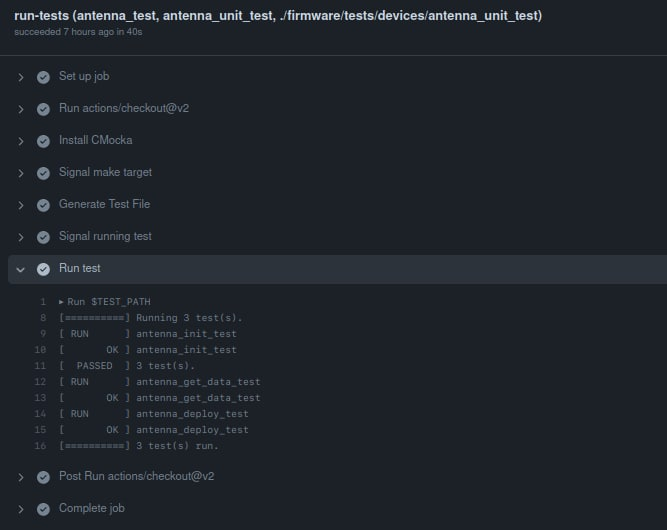
\includegraphics[width=\textwidth]{images/workflow_log.jpg}
                \label{fig:workflow-log}
                \legend{Fonte: OBDH 2 \cite{obdh2-github}}
            \end{figure}
            
            Os \textit{workflows} nos repositórios da missão são organizados em duas etapas distintas, separadas em Pré Execução \autoref{projeto:pre-exec} e Execução propriamente dita \autoref{projeto:exec}.
        
        \subsection{Pré Execução}
        \label{projeto:pre-exec}
            Na etapa de Pré Execução, são realizadas algumas tarefas para preparar o \textit{workflow}. Configurações iniciais, como escolha de sistema operacional e download e instalação de pacotes necessários foram omitidas, por se tratarem de configuração padrão da ferramenta, e não tem relevância para a execução do modelo desenvolvido.
            
            A primeira tarefa é a elaboração de uma \textit{Job Matrix}, que se trata de uma estrutura de dados empregada pela ferramenta para estabelecer um conjunto de \textit{jobs}, como são chamadas as ações da ferramenta. Um exemplo \textit{job}, no contexto do FloripaSat-II, seria um teste a ser executado. A \textit{Job Matrix} é utilizada, então, para dividir o \textit{workflow} de modo que cada arquivo de teste seja encapsulado em uma sub-tarefa distinta, que são executadas de maneira paralela. Optou-se por esse modelo como maneira de garantir execução e análise eficientes de e de maneira independente. A \autoref{tab:driver-tests} e a \autoref{tab:device-tests} apresentam uma comparação entre as execuções do workflow no repositório do OBDH 2.0 atual, e uma versão sequencial implementada especialmente para este teste.
            
            %%%%%%%%%%%%%%%TABELA%%%%%%%%%%%%%%%%%
\begin{table}[ht!]
\centering
\begin{tabular}{|l|l|l|l|}
\hline
\textbf{Modo de Execução  }    & \textbf{Min} & \textbf{Max}  & \textbf{Média} \\ \hline
Sequencial            & 38  & 69   & 50.27  \\ \hline
Paralela (Job Matrix) & 74  & 434\footnotemark & 128  \\ \hline
\end{tabular}
\caption{Tabela comparativa de tempos de exeução em segundos do workflow de testes unitários dos \textit{drivers} do OBDH 2.0}
\label{tab:driver-tests}
\end{table}
            %%%%%%%%%%%%%%%TABELA%%%%%%%%%%%%%%%%%
            
\begin{table}[ht!]
\centering
\begin{tabular}{|l|l|l|l|}
\hline
\textbf{Modo de Execução }     & \textbf{Min} & \textbf{Max} & \textbf{Média} \\ \hline
Sequencial            & 27  & 79  & 47.2  \\ \hline
Paralela (\textit{Job Matrix}) & 57  & 105 & 72.8  \\ \hline
\end{tabular}
\caption{Tabela comparativa de tempos de exeução em segundos do workflow de testes unitários dos \textit{devices} do OBDH 2.0}
\label{tab:device-tests}
\end{table}
        %%%%%%%%%%%%%%%TABELA%%%%%%%%%%%%%%%%%
        
            \footnotetext{O tempo de duração de 434 segundos foi possivelmente uma anomalia decorrente de alguma instabilidade na plataforma, visto que nenhuma das outras 10 execuções desse mesmo módulo apresentou valores próximos a este. Para fins de comparação, foi realizada uma nova medição desse mesmo workflow, e a média recalculada descartando o valor anômalo foi de 97.4 segundos. A lista completa das execuções pode ser encontrada nas tabelas \ref{tab:driver-tests-full} e \ref{tab:device-tests-full} no apendice \ref{apendice:tabelas}}
            
            O \textit{workflow} que implementa a execução sequencial dos testes se mostrou comparativamente mais rápido à execução paralela. A razão da escolha do uso da \textit{Job Matrix} foi a possibilidade de granularizar a execução, controlando de maneira individual se um teste deve ou não ser executado, além de ser possível analizar os resultados da execução de maneira individual. Como cada item da matriz é visualizada como um \textit{workflow} separado nos logs do GitHub, se torna trivial encontrar o teste desejado e analizar o resultado de sua execução. Na forma sequencial, por exemplo, a execução se dá em um único \textit{workflow}, e os testes e resultados devem ser buscados no log.
            
            Nesse contexto, um \textit{job} principal faz o levantamento de todos os arquivos de teste disponíveis para serem executados, e para cada arquivo é gerada uma entrada na \textit{job matrix}, de modo que cada teste seja compilado e executado em um \textit{job} isolado.
            
            O trecho de código \autoref{projeto:unit-test-devices} representa a seção do \textit{workflow} responsável por gerar o conteúdo da \textit{Job Matrix}, que no caso é populada com informações sobre os testes a serem executados.
            
            \lstinputlisting[language=yml, label={projeto:unit-test-devices}, caption=Geração da Job Matrix no workflow de autmação dos testes de \textit{devices} do OBDH, firstline=38, lastline=64]{code/unit-test-devices.yml}
            
            
            A execução desta etapa, que por sua vez invoca um script Python que lê o diretório onde o teste está implementado, cuja localização no repositório é informada no momento da execução. Assim, cada \textit{workflow} informa o caminho desejado. Por exemplo, no caso do OBDH 2.0, o workflow de \textit{drivers} informaria o caminho \texttt{firmware/tests/drivers}, enquanto o workflow de \textit{devices} deverá informar \texttt{firmware/tests/devices}. Essa configuração deve ser feita de forma manual na implementação dos \textit{workflows} individuais, e segue o padrão estabelecido e descrito na \autoref{proposta:padrao}.
            
            A execução deste script resultará em uma lista no formato \textit{.json} com os seguintes componentes:
            
            \begin{itemize}
                \item \textit{name}: o nome do arquivo de teste fonte.c, \textit{sem a extensão};
                \item \textit{test\_name}: o nome do executável após a compilação do arquivo fonte;
                \item \textit{path}: o diretório onde se encontra o executável;
            \end{itemize}
            
            Um exemplo desta lista gerada pelo workflow de \textit{devices} do OBDH 2.0 está disponível no trecho de código \autoref{projeto:test-list}.
            
            \lstinputlisting[language=json, label={projeto:test-list}, caption=Lista de testes gerada pelo script de identificação de arquivos, firstline=2, lastline=17]{code/test-list.json}
        
            O arquivo \textit{.json} apresenta o resultado da execução do script, onde cada elemento de \textit{include} é um dicionário contendo o nome do arquivo fonte, o nome e a localização do executavel.
            
            Esse arquivo é lido nos próximos passos do workflow para gerar os \textit{jobs} individuais com cada um desses dicionarios, dessa forma cada \textit{job} lida apenas com um executavel.
            
        \subsection{Execução}
        \label{projeto:exec}
            Após as configurações realizadas na etapa de Pré Execução, o \textit{workflow} realiza a compilação e a execução dos arquivos listados anteriormente, localizados no arquivo \textit{.json} gerado.
            
            Para efeitos de ilustração, assumiremos um commit na branch \textit{dev\_firmware} do repositório do OBDH 2 como evento \textit{e}, que aciona a execução de um \textit{worklow} \textit{w}.
            
            Após a etapa de Pré Execução, todos os arquivos de teste dos \textit{drivers} e \textit{devices} do OBDH2 estarão listados no arquivo \textit{.json}, e a \textit{Job Matrix} estará populada com os nomes e os caminhos de cada um deles. Cada entrada na matriz é, então, dividida em uma sub tarefa.
            
            Como cada tarefa é encarada como um \textit{workflow} distinto sob o ponto de vista de execução, todas elas precisam realizar algumas configurações iniciais como as descritas anteriormente, de download e instalação de bibliotecas. Após isso, o teste é compilado, e o binário gerado é executado. Ao final da execução, um registro com informações sobre o \textit{workflow} é gerado (\autoref{fig:workflow-log}).
            
            Caso algum dos testes apresente falha, o \textit{workflow} registrará um erro de execução, mas isso ocorrerá apenas após a finalização de todos os testes.
            
            A \autoref{fig:workflow_chart} ilustra um fluxo de execuções seguindo as etapas discutidas nas últimas seções.
            
            
\begin{figure}[h!]
    \centering
    \caption{Fluxo de execução do modelo de automação}
    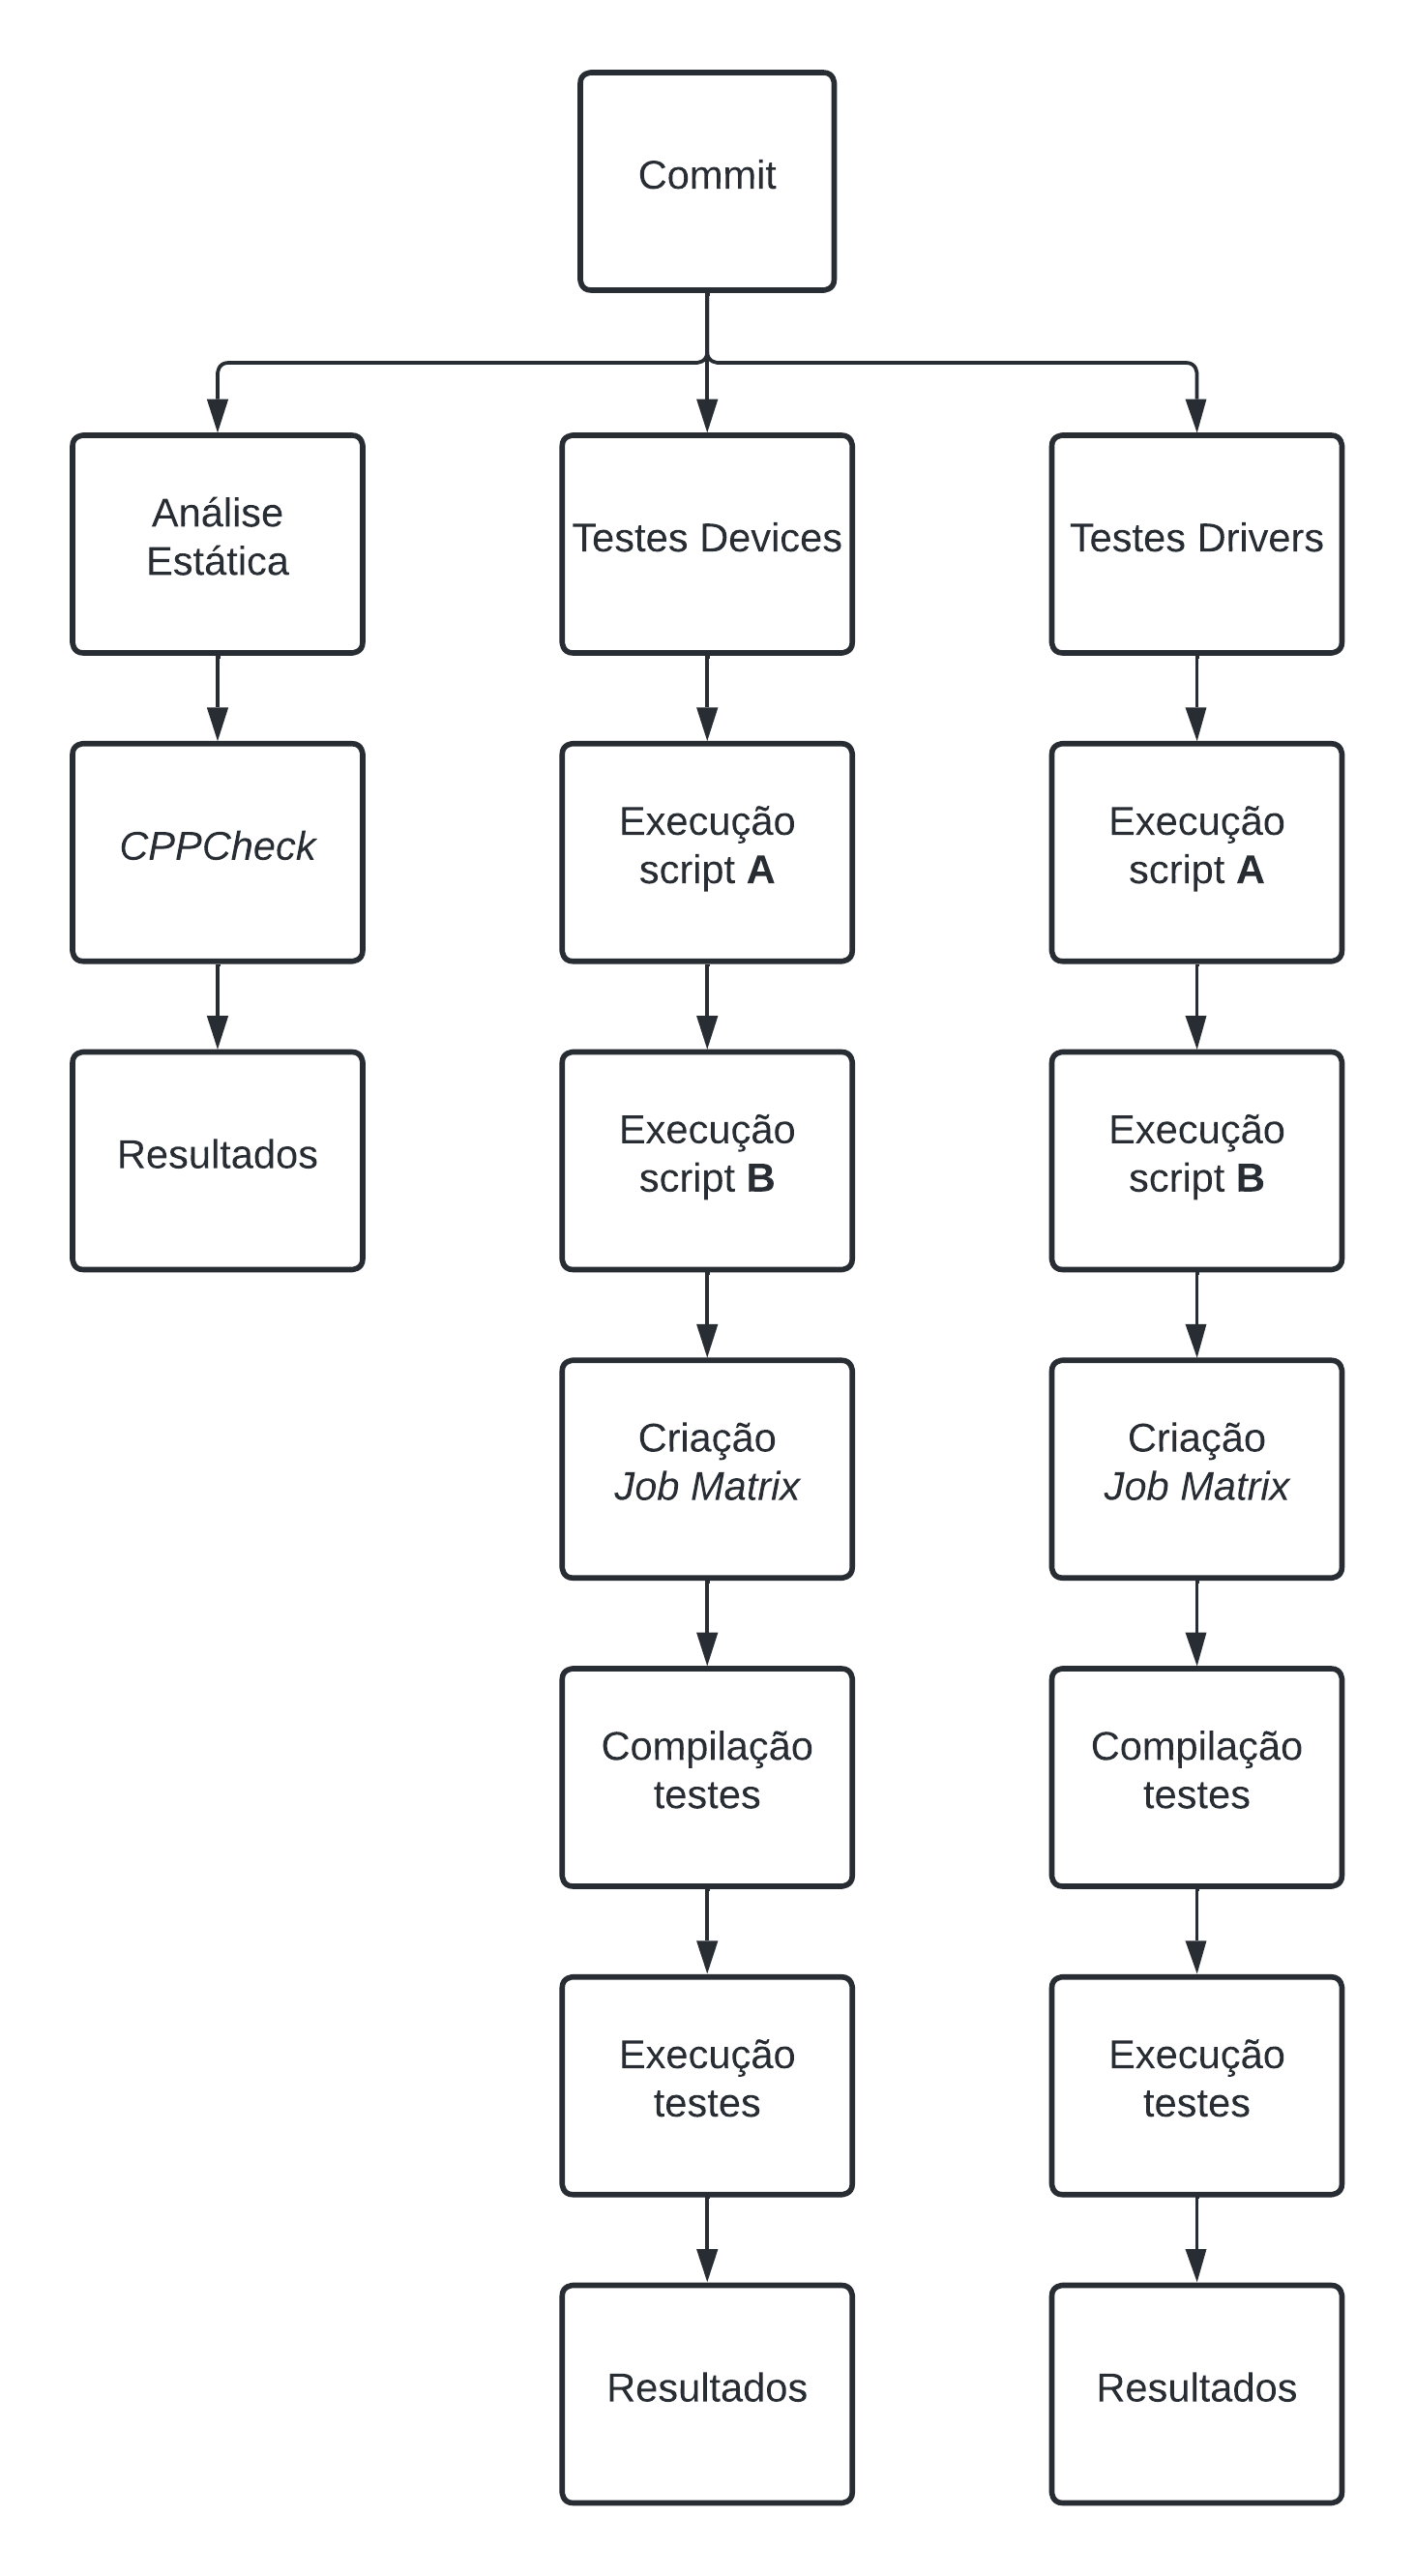
\includegraphics[scale=.15]{images/workflow_chart.png}
    \legend{Fonte: O autor}
    \label{fig:workflow_chart}
\end{figure}